\documentclass[11pt,a4paper]{ctexart}
\usepackage{ctex}
\usepackage{graphicx}
\usepackage{epstopdf}
\usepackage{xcolor}
\usepackage{amssymb}
\usepackage{amsmath}
\usepackage{amsfonts}
\usepackage{subfigure}
\usepackage{float}
\usepackage{cases}
\usepackage{cmap}
\usepackage{stfloats}
\usepackage{booktabs}
%\usepackage{cite}
\usepackage{ulem}
\usepackage{multirow}
\usepackage{titlesec}
\setcounter{table}{0}
\usepackage[CJKbookmarks,breaklinks=true]{hyperref}
\usepackage{cleveref}
\pagestyle{plain}
\topmargin=-1.5cm
\oddsidemargin=-0.55cm \evensidemargin=0pt
\textwidth=17cm
\textheight=25cm
\newtheorem{theorem}{定理}[section]
\newtheorem{definition}{定义}[section]
\usepackage{ulem} 
\usepackage[square, comma, sort&compress, numbers]{natbib}
\newcommand\dx{\,\mathrm{d}x}% 定义微分符号dx
\newcommand\dt{\,\mathrm{d}t}
\newcommand\dy{\,\mathrm{d}y}
\newcommand\dd{\,\mathrm{d}}
\newcommand\dint{\displaystyle \int} 
\newcommand\myciteup[1]{{\setcitestyle{square,super}\cite{#1}}}
\usepackage{caption}
\captionsetup{labelformat=default,labelsep=space} %去除冒号

% 参考文献
%\bibliographystyle{unsrt}
%\usepackage{gbt7714}
% 参考文献输出方式，numerical为按照出现顺序，authoryear为按照作者姓名和年份
%\bibliographystyle{gbt7714-numerical}

\begin{document}
\title{变系数YTSF方程的双线性形式与解析解}
\author{张一, 宋二}
\maketitle

\begin{abstract}
    本文的研究对象是在流体动力学、等离子体物理等方面有较为广泛应用的Yu-Toda-Sasa-Fukuyama\\
    (YTSF)方程，主要分析该方程的解析性质并求其精确解。利用 WTC 法考察了变系数 YTSF 方程的 Painlev\'{e} 性质，求得该方程的 Painlev\'{e} 可积条件；利用 Painlev\'{e} 截断方法计算变系数 YTSF 方程的自 B\"{a}cklund 变换，并基于此求得特殊孤子解和周期解；基于自 B\"{a}cklund 变换求得变系数 YTSF 方程的双线性方程，并由此得到多孤子解。最后我们对所得的解进行图像绘制和物理性质分析。
\end{abstract}

\textbf{关键词}：变系数YTSF方程，Hirota双线性方法，Painlev\'{e}性质，自B\"{a}cklund变换

\section{引言}

1998年，Yu, Toda, Sasa, Fukuyama 四人在利用三线性形式研究(2 + 1)维的 Bogoyavlenskii-Schiff 方程时，利用强对称性提出了一个新的(3+1)维方程—— Yu-Toda-Sasa-Fukuyama 方程，简称为 YTSF 方程\cite{1,2,3}:
\begin{equation}
    [\Phi(\eta)\eta_z-4\eta_t]_{\xi}+3\eta_{yy}=0,\label{1y}
\end{equation}
\begin{equation}
    \Phi(\eta)=\partial_{\xi}^2+4\eta+2\eta_{\xi}\partial_{\xi}^{-1},
\end{equation}
其中$\eta$是“时间变量”$t$和“空间变量”$\xi,y,z$的函数，表示波的振幅\cite{4,5}。
在物理应用中，YTSF 方程描述了晶格中的弹性准平面波或两层液体中的界面波，反映了简化系统的反应混合物和浅水方程的势能。YTSF 方程体现了浅水处水的形态运动与在该形态上传播的波的尺度相对应，被用于研究流体动力学、等离子体物理、弱色散介质中孤子和非线性波的动力学等方面的问题，对这些领域的发展有着很大的帮助\cite{6}。

如果使$\eta=u_{\xi},\xi-z \rightarrow x,y \rightarrow y,t\rightarrow t$，则方程(\ref{1y})可转化为一个(2+1)维的简化YTSF方程，具体形式如下：
\begin{equation}
    -4u_{xt}-u_{xxxx}-6u_xu_{xx}=0,\label{2y}
\end{equation}
其中$u$是$x,y$和$t$的函数。

本文以上述常系数(2+1)维YTSF方程\eqref{2y}为基础,研究了推广的变系数YTSF方程
\begin{equation}
    u_{xt}+a_1(t)u_xu_{xx}+a_2(t)u_{xxxx}=0,
\end{equation}
其中$a_1(t),a_2(t),a_3(t)$是关于$t$的可微函数。


1971年，日本数学家 Hirota 基于反散射方法提出双线性方法，其主要思想是将一个非线性发展方程通过某种变换化成一个或多个双线性方程，其所有项都是二次，然后将扰动展开式代入双线性方程中，通过截断展开式进行求解，可得单孤子解、双孤子解等，并基于此可通过数学归纳法得N-孤子解的表达式。

Hirota双线性方法提出后，很快求得了KdV方程、mKdV方程、KP方程等的孤子解。除此以外，基于双线性方程还能求得非线性偏微分方程的周期解、有理解等。但双线性方法较为困难，并不适用于所有非线性发展方程。近年来，诸多学者致力于双线性方法的应用和推广，在一定程度上促进了该方法的完善和拓宽。

\begin{definition}\label{d1}
    x的m阶t的n阶双线性算子{\rm \cite{pzl1998}}：
    \begin{align*}
        D_x^mD_t^na \cdot b & \equiv (\frac{\partial}{\partial x}-\frac{\partial}{\partial y})^m(\frac{\partial}{\partial t}-\frac{\partial}{\partial s})^n a(x,t)b(y,s)\bigg|_{y=x,t=s} \\
                            & =\frac{\partial^m}{\partial y^m}\frac{\partial^n}{\partial s^n}a(x+y,t+s)b(x-y,t-s)\bigg|_{y=0,s=0}                                                        \\
                            & =\sum_{j=0}^{n}(-1)^j{ n \choose j }\sum_{i=0}^{m}(-1)^i{ m \choose i }a^{(m-i,n-j)}b^{(i,j)}.
    \end{align*}
    其中$a(x,t),b(x,t)$是关于变量$x,t$的具有任意阶导数的两个函数，$a^{(i,j)}=\dfrac{\partial^{i+j} a}{\partial x^i\partial t^j}$，m和n是正整数。
\end{definition}

%本文的主要研究内容如下：在第2节中对变系数YTSF方程进行Painlev\'{e}性质检测；在第3节中构造变系数YTSF方程的自B\"{a}cklund变换并求特殊解；在第4节中求变系数YTSF方程的双线性形式，并基于此求多孤子解；最后在第5节中设置特殊参数对求得的多孤子解进行图像绘制，分析孤子解的性质。

\section{变系数YTSF方程的Painlev\'{e}性质}
Painlev\'{e} 分析是研究非线性发展方程的一个十分重要的方法，既可以用来判断方程的可积性，又可以用来求方程的解析解。因此在本节中我们利用 WTC 法对变系数YTSF方程进行Painlev\'{e} 检测。



\section{变系数YTSF方程的双线性形式与多孤子解}

Hirota 双线性方法是求非线性微分方程解析解的一类重要的直接方法，本节中我们利用此方法对变系数 YTSF 方程进行求解。基于Painlev\'{e}检测和自B\"{a}cklund变换，我们考虑方程\label{2y}的一种特殊情况，取$a_1(t)=ca_2(t)$\,($c$为任意常数)，此时变系数YTSF方程的形式：
\begin{equation}
    u_{xt}+ca_2(t)u_xu_{xx}+a_2(t)u_{xxxx}+a_3(t)u_{yy}=0,\label{3tsy}
\end{equation}
求该方程的双线性形式和多孤子解。
\subsection{双线性方程}
对自B\"{a}cklund变换得到的$u$的表达式，取种子解$u_1(x,y,t)=0$，得：


\subsection{多孤子解}
记算子$B=D_xD_t+a_2(t)D_x^4+a_3(t)D_y^2$，则原方程的双线性形式为
\begin{equation}
    B\phi \cdot \phi=0.
\end{equation}
令
\begin{equation}
    \phi(x,y,t)=1+\sum_{i=1}^{\infty}\varepsilon^iF_i(x,y,t),
\end{equation}
则
\begin{equation}
    B(1\cdot 1)+\varepsilon B(1\cdot F_1+F_1\cdot 1)+\cdot \cdot \cdot+\varepsilon^rB\bigg(\sum_{m=0}^{r}F_{r-m}\cdot F_m \bigg)+\cdot \cdot \cdot=0.
\end{equation}
令$\varepsilon$ 的各次幂的系数为零，可得：
\begin{equation}
    B(F_1)=0,\label{3s1}
\end{equation}
\begin{equation}
    B(F_2)=-\frac{1}{2}B(F_1 \cdot F_1),\label{3s2}
\end{equation}
\begin{equation}
    B(F_3)=-B(F_1 \cdot F_2),\label{3s3}
\end{equation}
\begin{equation}
    B(F_4)=-\frac{1}{2}B(2F_1 \cdot F_3+F_2 \cdot F_2),
\end{equation}
\begin{equation*}
    \cdots \cdots
\end{equation*}



再令$F_i=0\,(i=4,5\cdot \cdot \cdot)$，$\varepsilon =1$，则
\begin{equation}
    \phi=1+\text e^{\theta_1}+\text e^{\theta_2}+\text e^{\theta_3}+a_{12}\text e^{\theta_1+\theta_2}+a_{13}\text e^{\theta_1+\theta_3}+a_{23}\text e^{\theta_2+\theta_3}+b\text e^{\theta_1+\theta_2+\theta_3}.
\end{equation}
将$\phi$代入\eqref{3zz}可得原方程的三孤子解。

\section{结论与讨论}

本文主要基于 Hirota 双线性方法对(2+1)维变系数 YTSF 方程进行了性质研究和特殊解求解。利用 WTC 法对上述方程进行 Painlev\'{e} 检测，可知变系数 YTSF 方程一般不具有 Painlev\'{e} 可积性，只有当变系数之间存在某种联系时，才能通过 Painlev\'{e} 检测。通过符号计算，我们得到变系数 YTSF 方程的一个自 B\"{a}cklund 变换，并且在此基础上求出了特殊孤子解和周期解。利用 Hirota 双线性方法将原方程化为双线性方程后，我们得到原方程的双线性形式，随后通过 Hirota 双线性形式求得了多孤子解。我们发现与单孤子解相比，在讨论双孤子解和三孤子解的过程中对变系数的要求更高。最后，我们设置不同的参数对求得的特殊解绘制三维图像，通过分析参数变化引起的图像变化体现孤子解的性质及应用价值。

由我们求出的变系数YTSF方程的特殊解，我们选取特殊参数对部分孤子解进行图像绘制，并对参数进行定性分析。

\noindent\textbf{Case 1}\quad 令函数系数为$a_1(t)=a_2(t)=a_3(t)=t$，并在$x,t$平面绘制关于$u$的图解，图\ref{p1}-图\ref{p3}中分别为单孤子解、双孤子解与三孤子解的图像，体现了$a_1(t),a_2(t),a_3(t)$均为$t$的线性函数时多孤子解的相互叠加作用,其中参数分别为：


$(1)l=\frac{3}{2},r=1;$

$(2)l_1=\frac{3}{2},l_2=-2,r_1=r_2=1;$

$(3)l_1=\frac{3}{2},l_2=-2,l_3=1,r_1=r_2=r_3=1.$



\noindent\textbf{Case 2}\quad 在$x,t$平面绘制关于$u$的图解，图\ref{p4}-图\ref{p6}中分别为单孤子解、双孤子解与三孤子解的图像，体现了变系数$a_1(t),a_2(t),a_3(t)$中有关于$t$的非线性函数时多孤子解的相互叠加作用，其中方程变系数及参数分别为：


$(1)a_1(t)=a_2(t)=t,a_3(t)=t^2,l=1,r=1;$

$(2)a_1(t)=a_2(t)=a_3(t)=t^2,l_1=\frac{3}{2},l_2=-2,r_1=r_2=1;$

$(3)a_1(t)=a_2(t)=a_3(t)=t^2,l_1=\frac{3}{2},l_2=-2,l_3=1,r_1=r_2=r_3=1.$


\begin{figure}[htbp]
    \centering
    \begin{minipage}[h]{0.325\textwidth}
        \centering
        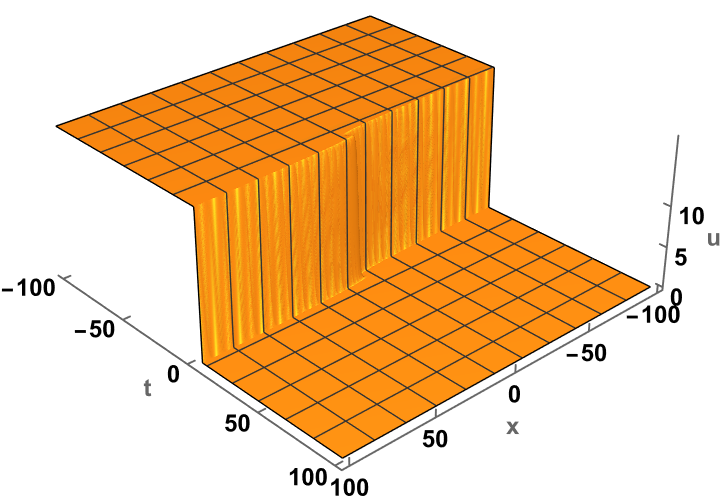
\includegraphics[width=0.8\linewidth]{ p7}
        \caption{}
        \label{p4}
    \end{minipage}
    \begin{minipage}[h]{0.325\textwidth}
        \centering
        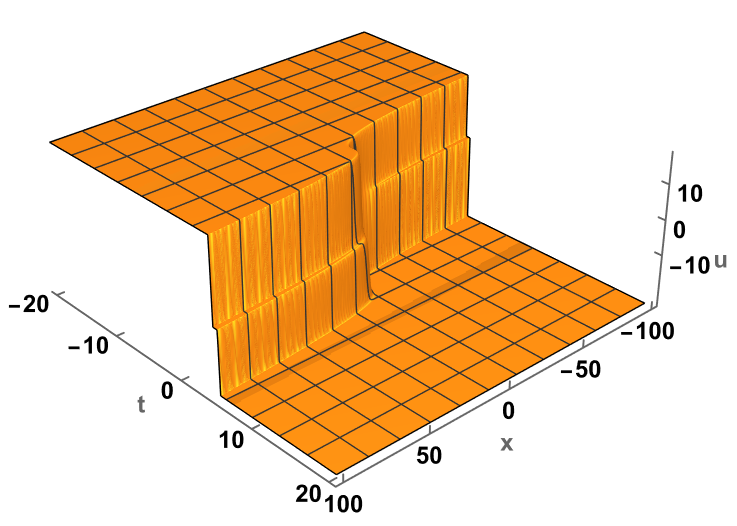
\includegraphics[width=0.8\linewidth]{ p8}
        \caption{}
        \label{p5}
    \end{minipage}
    \begin{minipage}[h]{0.325\textwidth}
        \centering
        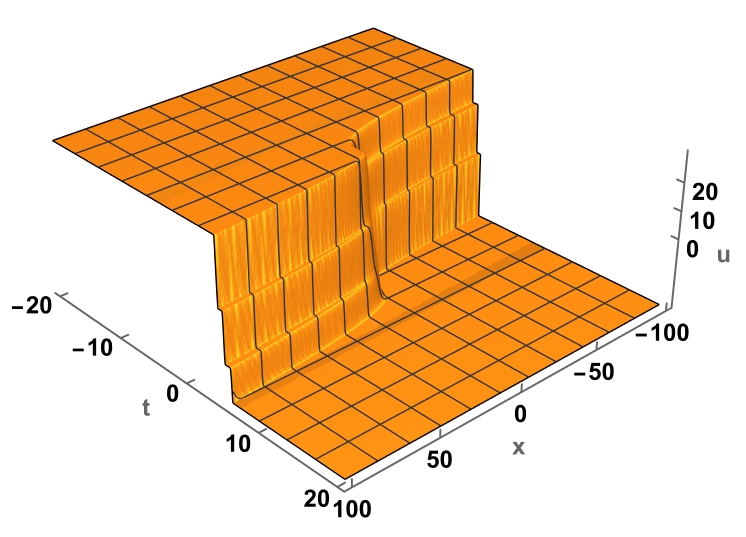
\includegraphics[width=0.8\linewidth]{ p9}
        \caption{}
        \label{p6}
    \end{minipage}
\end{figure}

\noindent\textbf{Case 3}\quad 在$x,t$平面绘制关于$u$的图解，图\ref{p4}-图\ref{p6}中分别为单孤子解、双孤子解与三孤子解的图像，体现了变系数$a_1(t),a_2(t),a_3(t)$中含$t$的周期函数时解的作用,其中方程变系数及参数分别为：




%\cleardoublepage
%\phantomsection
%\addcontentsline{toc}{chapter}{参考文献}
%\nocite{*} %排版所有包括未引用的文献
%\bibliography{bibs}
%\cleardoublepage

\begin{thebibliography}{9}
    \bibitem{1}
    高普云.  非线性动力学[M]. 长沙\,: 国防科技大学出版社, 2005\,: 2-9

    \bibitem{2}
    张建树, 孙秀泉, 张正军. 理论力学[M]. 北京\,: 科学出版社, 118,
    236-239

    \bibitem{3}
    郭柏灵. 非线性演化方程[M].  上海\,: 上海科技教育出版社, 1998\,: 5,
    180

    \bibitem{4}
    倪皖荪， 魏容爵. 水槽中的孤波[M]. \, 上海\,: 上海科技教育出版社,
    1997\,: 98, 104

    \bibitem {5}
    Infeld E., Rowlands G. Nonliear Waves, Solitons and Chaos[M]. Second
    Edition.  Cambridge\,: Cambridge University  Press, 2000\,: 5-9

    \bibitem {6}
    Remoissenet M.  Waves Called Solitons[M]. Second Edition. Beijing\,:
    World Publishing Corporation, 1999\,: 182, 202

\end{thebibliography}

\title{The Bilinear Equation and Analytical Solutions of the Variable-coefficient Yu-Toda-Sasa-Fukuyama Equation}
\author{SONG Yu-xin,WEI Guang-mei\\
}
\maketitle

\noindent \textbf{Abstract}Yu-Toda-Sasa-Fukuyama(YTSF) equation is investigated in this paper, which has been widely used in fluid dynamics and plasma physics, etc. The main research contents are the analytic property and exact solutions of this equation. According to a (2+1)-dimensional YTSF equation with fixed constant coefficients , we discuss the Painlev\'{e} property, auto-B\"{a}cklund transformations and bilinear forms of the variable-coefficient YTSF equation. For this equation, the Painlev\'{e} property is analyzed by WTC method, and then the special soliton solution and periodic solution are obtained from auto-B\"{a}cklund transformation. Then the bilinear form of the original equation is constructed with Hirota bilinear method, and we get the single soliton solution, double soliton solution and triple soliton solution from the bilinear equation. In the end, for the special solutions of the equation, we set different parameters to draw the images of the solutions and analyze them.

\noindent \textbf{Keywords}: Variable-coefficient Yu-Toda-Sasa-Fukuyama equation, Hirota bilinear method, Painlev\'{e} property, Auto-B\"{a}cklund transformation, Analytical solution

\end{document}